\section{Relational Data Model}
We describe the relational data model in this section. It is the foundation of the search problem that is studied in this thesis.  

Let $R$ be a relation and $\Attr(R)$ be the attributes of $R$. The attributes are a set of names.  Each tuple of $R$ is
a function that maps attributes of $R$ to values:
$$
t : \Attr(R) \to \Values
$$
The relation $R$ is a set of such tuples:
$$
R = \{t_1, t_2, \dots, t_n\}
$$

\begin{example}
Consider a table shown below:
\begin{center}
    \centering
    \begin{tabular}{|c|c|}\hline
    {\bf Name} & {\bf Address} \\ \hline
    Jack & 100 Simcoe Street \\ \hline
    Jill & 56 Taunton Road \\ \hline
    Joe & 5 Collin Road \\ \hline
    \end{tabular}
\end{center}
The attributes are:
$$ \Attr(R) = \{\mathrm{Name}, \mathrm{Address}\} $$
The relation consists of three tuples:
$$ R = \{t_1, t_2, t_3\} $$
where $t_1$ is a mapping given by:
$$
t_1 = \left[\begin{array}{rcl}
\mathrm{Name} & \mapsto & \makebox{Jack} \\
\mathrm{Address} & \mapsto & \makebox{100 Simcoe Street} \\
\end{array}\right]
$$
The other two tuples, $t_2$ and $t_3$, are defined similarly.
\end{example}

A relational database will have more features added to its relational model. For example,
\begin{itemize}
    \item Primary keys and foreign keys
    \item Dependencies and constraints
    \item Structured query language (SQL)
\end{itemize}
More details can be found in texts such as García-Molina et al  \cite{garcia2005database}.  However, in the context of our thesis, we do not rely on these additional features of a relational model.  More precisely, the relational model we focus on is the first normal form \cite{beeri1979computational}.

\section{Document Models}
While the relational model is widely used, it does have limitations. One such limitation is the lack of flexibility of its schema, namely, all tuples of the same relation {\em must} have the same set of attributes.

Text search engines popularized the document model \cite{croft2010search}. It supports schema-less data management.  In the document model, a document is defined as
a mapping from {\em fields} to text values.

\subsection{Documents}
Let $d$ be a document and $\Attr(d)$ be its set of fields. The fields $\Attr(d)$ is a set of names, similar to the attributes of a relation.
The document $d$ is a function that maps fields to text:
$$ d : \Attr(d) \to \mathbf{Text} $$

A document collection is denoted by $D = \{d_1, d_2, \dots, d_n\}$.
It's important to note that a document collection is fundamentally different from a relation, that is, 
\begin{center}
    different documents $d, d'\ (d\not=d')$ can have different fields:
$\Attr(d)\not=\Attr(d')$.
\end{center}

\begin{example} \label{ex2}
Consider three documents in a document collection $D$. The first has two fields: $Name$ and $Address$. It can be denoted as:
$$
d_1 = \left[\begin{array}{rcl}
\mathrm{Name} & \mapsto & \makebox{Jack} \\
\mathrm{Address} & \mapsto & \makebox{100 Simcoe Street} \\
\end{array}\right]
$$

The second has three fields: $Name$, $Occupation$, and $Address$. It can be denoted as:
$$
d_2 = \left[\begin{array}{rcl}
\mathrm{Name} & \mapsto & \makebox{Jack} \\
\mathrm{Occupation} & \mapsto & \makebox{Student} \\
\mathrm{Address} & \mapsto & \makebox{100 Simcoe Street} \\
\end{array}\right]
$$

The third has four fields: $Restaurant\ Name$, $City$, $Rating$, and $Comment$. It can be denoted as:
$$
d_3 = \left[\begin{array}{rcl}
\mathrm{RestaurantName} & \mapsto & \makebox{The Best Grill} \\
\mathrm{City} & \mapsto & \makebox{Oshawa} \\
\mathrm{Rating} & \mapsto & \makebox{5} \\
\mathrm{Comment} & \mapsto & \makebox{very nice place} \\
\end{array}\right]
$$
\end{example}

\subsection{Tokenization}

The main objective of the document model is to support keyword search efficiently.  This involves searching for documents whose fields contain certain sub-strings, which we call {\em tokens}.  The process of token generation is referred to as tokenization (also known as lexical analysis).  Tokenization is an important step in natural language processing \cite{jimenez2018impact,kudo2018sentencepiece}, especially for non-English languages \cite{takaoka2018sudachi,cao2011research}.

Before we can store the documents, we first need to transform text values into lists of tokens.  We do this by using a tokenizer:
$$
\mathbf{tokenize} : \mathbf{Text} \to \List[\Token]
$$

Given a document $d$, a {\em term} is a field-token pair that is derived from the result of tokenzing the text value of a field.
Then the term set of a document $d$ is given by:
$$
\mathbf{termset}(d) = \{
  (f, x): f\in\Attr(d),\ x\in\mathbf{tokenize}(d(f))
\}
$$

Given a document collection $D$, a simple document query is to find all documents with a specific term: $term^* = (f^*, x^*)$.  The answer set to the query is given as:
$$\mathbf{answerset}(D, term^*) = \{d\in D: term^*\in\mathbf{termset}(d)\}$$

\begin{example}
Consider the above three documents in the document collection $D$ of Example \ref{ex2}. If we search field ``Address" by keyword ``Simcoe", the search query is:
$$term^* = (Address, Simcoe)$$. 
The answer set will be:
$$\mathbf{answerset}(D, term^*) = \{d1, d2\}$$

\end{example}

\subsection{Keyword queries and matching scores}

Internet search engines made keyword queries as a standard way of accessing text documents \cite{ntoulas2004s}.
Important aspects of keyword queries are:
\begin{itemize}
    \item There is no fixed syntax: queries can be as simple as a phrase or a piece of plain text.
    \item The search results do not need to match the query perfectly. They are ranked by some matching scores instead.
\end{itemize}

A {\em keyword query} is a text, annotated by a field name.
$$Q = (f_q, q)$$
where $f_q$ is a field name, and $q\in\mathbf{Text}$.

The matching between the query $Q = (f_q, q)$ and the documents in a collection $D$ is determined by the matching of their respective termsets.  The termset of the query is defined as:
$$
\mathbf{termset}(Q) = \{(f_q, x): x\in\mathbf{tokenize}(q)\}
$$

\newcommand{\Termset}{\mathbf{termset}}
\newcommand{\TFIDF}{\mathbf{TFIDF}}
A natural matching score between $Q$ and some document $d$ is the overlap between their termsets.  The Jaccard similarity measures a normalized overlap as defined as:
$$
\mathrm{sim}(Q, d) = \frac{|\Termset(Q)\cap\Termset(d)|}{|\Termset(Q)\cup\Termset(d)|}
$$

Jaccard similarity is sufficient in many document retrieval scenarios. However, it is not the ideal measure for documents based on natural languages. There are many words in the vocabulary of natural language text that have overwhelming high frequencies, for example, {\em the}, {\em a}, {\em this}, etc.  Their occurrences should be discounted towards the similarity score.  {\em Term frequency-inverse document frequency} (tf-idf) measure is a term-normalized score better suited for natural language based query-document matching.

Each term $t\in\Termset(d)$ in a document $d$ has a weight, known as its tf-idf weight, defined as follows.

Denote the number of occurrences of $t$ in $d$ as $\#(t,d)$.  The term frequency is the normalized number of occurrences of $t$:
$$
\mathrm{TF}(t, d) = \frac{\#(t, d)}{\sum_{x\in\Termset(d)}\#(x, d)}
$$
In order to discount frequent words, we also compute the {\em inverse document frequency} of $t$ with respect to the entire document collection $D$:
$$
\mathrm{IDF(t)} = \log \frac{|D|}{|\{d\in D: t\in\Termset(d)\}|}
$$
Note that $\mathrm{IDF}(t)$ is inversely proportional to the popularity of a word.  Frequently occurring words have lower IDF weights.

Finally, the TF-IDF weight is the produce:
$$
\TFIDF(t, d) = \mathrm{TF}(t, d)\cdot \mathrm{IDF}(t)
$$

If a term $t$ does not appear in a document $d$, then its TF-IDF weight is zero.  Each document and query can be seen as a (sparse) vector of TF-IDF weights, and their matching score is measured by the cosine similarity of their TF-IDF vector representation.
\begin{equation}
\mathrm{sim}(Q, d) = \frac{\sum_{x}\TFIDF(x, Q) \TFIDF(x,d)}{
\sqrt{\sum_{x}\TFIDF(x,Q)^2 \sum_{y}\TFIDF(y,d)^2}
}
\label{eq:tfidf-sim}
\end{equation}

Equation~\ref{eq:tfidf-sim} provides an unbiased measure of similarity between the termsets of the query and a document by discounting frequently occurring words.

\section{Document Indexes and Search Engines}
In the previous section, we have defined a number of similarity measures which can be used to rank {\em all} documents with respect to a user defined query.

A search engine needs to efficiently identify the top-$k$ matching documents using some similarity score.  A naive approach would require evaluating the similarity score of all the documents, which has a data complexity of $\mathcal{O}(n)$, where $n$ is the total number of documents.  For large document corpora, search engines need better algorithms for keyword query processing.

\newcommand{\Id}{\mathbf{id}}
\newcommand{\Idset}{\mathbf{idset}}

The most widely used data structure for keyword search is the {\em inverted term index}. 
Let $D$ be a document collection. The term set of $D$ is given by,
$$
\Termset(D) = \{\Termset(d):  d \in D\}
$$
Let $\Id(d)$ be the id of a document $d$. The inverted term index is a function mapping terms to lists of document ids,
$$
\mathbf{index} : \Termset(D) \to \List[\Id(d): d \in D]
$$

\begin{example}
Consider the three examples in Example \ref{ex2}. The inverted term index can be denoted as,
$$
\left[\begin{array}{rcl}
	\mathrm{(Name, Jack)} & \mapsto & \makebox{\{d1, d2\}}  \\
	\mathrm{(Address, 100)} & \mapsto & \makebox{\{d1, d2\}}  \\
	\mathrm{(Address, Simcoe)} & \mapsto & \makebox{\{d1, d2\}}  \\
	\mathrm{(Address, Street)} & \mapsto & \makebox{\{d1, d2\}}  \\
	\mathrm{(Occupation, Student)} & \mapsto & \makebox{\{d2\}}  \\
	\mathrm{(RestaurantName, The)} & \mapsto & \makebox{\{d3 \}}  \\
	\mathrm{(RestaurantName, Best)} & \mapsto & \makebox{\{d3 \}}  \\
	\mathrm{(RestaurantName, Grill)} & \mapsto & \makebox{\{d3 \}}  \\
	\mathrm{(City, Oshawa)} & \mapsto & \makebox{\{d3\}}  \\
	\mathrm{(Rating, 5)} & \mapsto & \makebox{\{d3\}}  \\
	\mathrm{(Comment, very)} & \mapsto & \makebox{\{d3\}}  \\
	\mathrm{(Comment, nice)} & \mapsto & \makebox{\{d3\}}  \\
	\mathrm{(Comment, place)} & \mapsto & \makebox{\{d3\}}  \\
\end{array}\right]
$$
\end{example}

\subsection{Keyword query performance}
Inverted term index \cite{putz1991using}, as illustrated in Figure \ref{fig:inverted_term_index}, has two main components: a dictionary and lists of document ids.
\begin{figure}
    \centering
    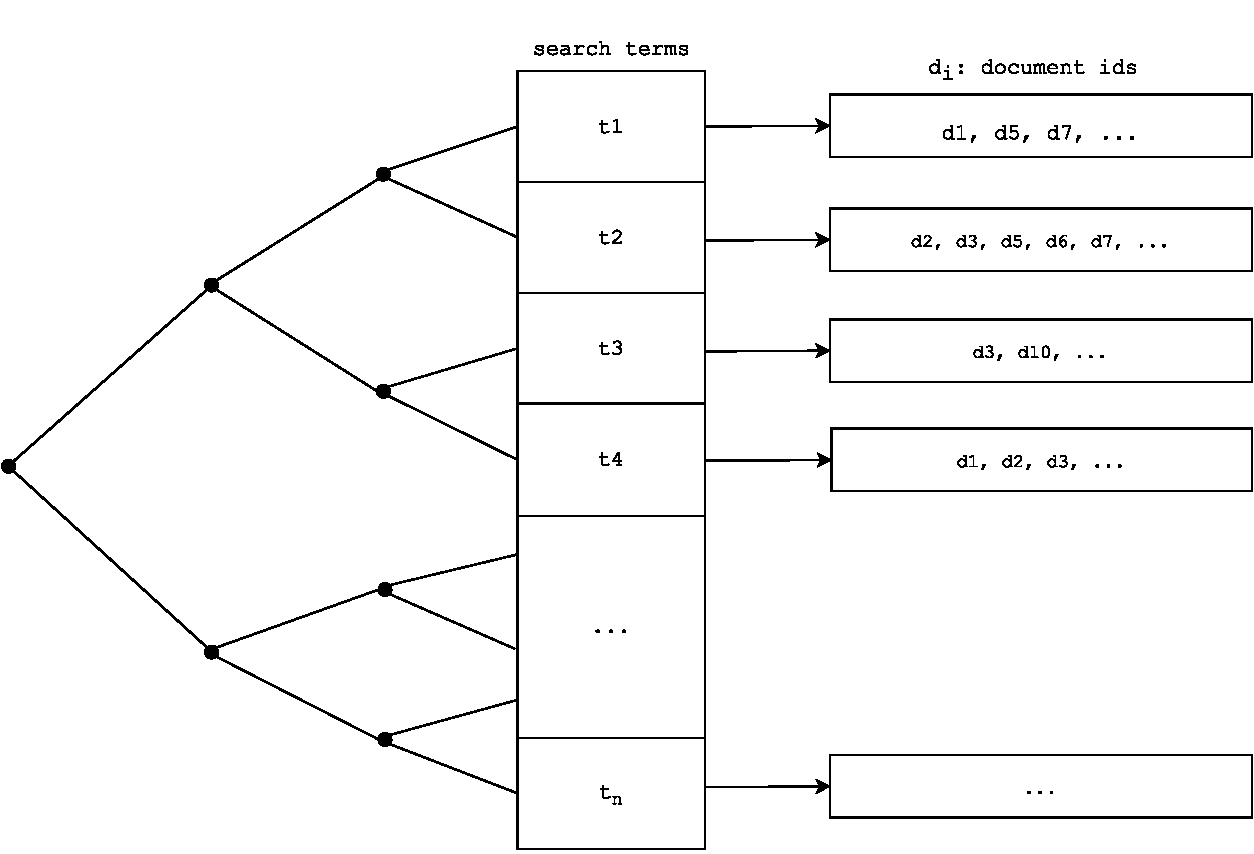
\includegraphics[width=0.7\textwidth]{my/chapters/background/figures/inverted-term-index.dio.svg.pdf}
    \caption{Inverted Term Index}
    \label{fig:inverted_term_index}
\end{figure}

We use the dictionary to look up a search term. After that, we retrieve the list of document ids associated with the term. Therefore, the query performance is determined by looking up terms of the query in the dictionary and merging all matched document id lists.

Let $q = <t_1, t_2, \dots, t_k>$ be a query, where $t_i$ are terms and $k$ is the number of terms of the query. The average length of document id lists is denoted as $l$. The total number of terms in the inverted index is denoted as $N$. Looking up a term $t_i$ has $\mathcal{O}(\log N)$ complexity. Merging matched document lists requires linear scan, which has $\mathcal{O}(k \times l)$ complexity . Therefore, the time complexity of processing the query is $\mathcal{O}(k \times \log N) + \mathcal{O}(k \times l)$.

\subsection{Fuzzy string matching and collisions}
\label{sec:fuzzy-collision}
A particularly important feature of keyword search based information retrieval is {\em fuzzy string matching}.  A common practice in performing fuzzy string matching based on the {\em n-grams} of the text \cite{kim1994fast}.

\begin{definition}[n-grams]
Let $s$ be a string where $s(i)$ is the $i$-th character from some alphabet $\Sigma$.  Let $n\geq 1$ be an
integer.  The $n$-padded string of $s$ is obtained by prepending and appending $n-1$ special symbols to $s$, defined as:

$$
s' = \underbrace{\mathtt{'\$'}\dots \mathtt{'\$'}}_{n-1\ \mathrm{times}} \cdot s\cdot
\underbrace{\mathtt{'\$'}\dots \mathtt{'\$'}}_{n-1\ \mathrm{times}} 
$$

The $n$-gram of $s$ is the set of strings of length $n$ defined as:
$$
\mathrm{G}_n(s) = \{s'(i) \dots s'(i+n-1): 1\leq i\leq |s'|-n+1\}
$$
\end{definition}

By definition, $G_n(s)\subseteq(\Sigma\cup\{\$\})^n$, namely all of its segments of length $n$ including
the padded special character $\$$.

\begin{example}
    Suppose that $s = \mathtt{``computer''}$.  Its 3-grams are given as:
    $$
    G_3(s) = \{
    \mathtt{\$\$c, \$co, com, omp, mpu, put, ute, ter, er\$, r\$\$}
    \}
    $$
\end{example}

Since $G_n(s)$ is a set that is derived from the content of $s$, we can
use it as a feature to compare strings in an approximate way.

\begin{definition}[Jaccard Similarity]
    Given two sets $A$ and $B$, their Jaccard similarity
    is given by:
    $$ J(A, B) = \frac{|A\cap B|}{|A\cup B|}$$

    Note $0\leq J(A, B)\leq 1$, with $J(A, B) = 1$ if and only if $A=B$.
\end{definition}

Using Jaccard similarity (and its derivatives), we can introduce
a similarity measure over strings.  Given two strings $s_1$ and $s_2$, the Jaccard similarity of the two strings is given by:
$$ J(s_1, s_2) = J(G_n(s_1), G_n(s_2)) $$

Now we can perform fuzzy string search using Jaccard similarity over strings. We index documents by storing their n-gram sets. The inverted index, therefore, will have n-gram tokens.
We also break all queries into n-gram sets for searching. Commonly 3-grams yield the best trade-off for the English language.

Recall that the inverted term index maps tokens to documents.  When 3-gram tokens are used, the total possible number of distinct tokens are given by
$|\Sigma|^3$. For the English language, $|\Sigma|\simeq 50$ (based on ASCII encoding).  So, there will only be $50^3 = 125,000$ possible tokens.  But, at the same time, a typical text index needs to support up to billions of documents.  As the number of documents exceeds the number of possible tokens, we run into the bad situation of severe collisions, which degrades the performance
from log-time $\mathcal{O}(\log n)$ to sequential scan $\mathcal{O}(n)$.

In this thesis, we will encounter the bottleneck of collision when 3-grams are used as tokens.  We will study methods involving partitioning the index, and optimizing index access pattern so that the search speed is improved.  Our optimization method will involve neural networks to learn the optimal access patterns using self-supervised learning.

In subsequent sections, we will review some elements of neural network design that are necessary to construct our embedded networks.

\section{Learning with neural networks}
\label{sec:neural-networks}
A neural network allows us to find patterns based on its training data. A trained neural network is an approximation of a function that maps its input data to its output data. In the context of this thesis, we explore ways to design neural networks as classifiers that will map partial tuple search queries to the relations that contain the tuples.


\subsection{General framework of machine learning}

The general framework of machine learning consists of three main components: representation of training data, a trainable model, and an optimization algorithm \cite{lecun2015deep,bengio2017deep}.

There are different types of data that can be used for machine learning, such as numerical data, text documents, images, and so on. They have to be converted to some format before they can be consumed by a machine learning model. In natural language processing, we use embedding vectors, which are numerical vectors, to represent texts \cite{li2018word,tripathy2021comprehensive}.

Fundamentally, the problem that machine learning (ML) is addressing must be modeled as a function:

$$
f : X \to Y
$$
where $X$ is a vector space that is the encoding of the input objects, and $Y$ is the output (usually also a vector space).  In the context of machine learning, the exact form of $f$, either mathematically or computationally, is not available.  However, we assume that we have many observations of the input-output pairs $\{(x_i, y_i): i=1\dots n\}$ of $f$.  The collection of $(x,y)$ pairs is known as the {\em training data}.

A trainable model is an algorithm that can learn from the training data. In the case of a neural network model, we define its structure by layers. We specify the number of layers the model consists of, the layer types, the number of neurons in each layer, and the connections between layers. The network structure determines the capabilities of the model.

We highlight the following  layer architectures that are used in this thesis.

\begin{itemize}
    \item Embedding layer: this layer architecture converts discrete and categorical inputs to dense vectors using a {\em hard coded} lookup table
    that maps tokens from a vocabulary to embedding vectors.  We will discuss this in more detail in Section~\ref{sec:embedding-layer}. The parameters
    of the embedding layer store the lookup table.
    \item Linear layer: this is the layer that is capable of performing linear separation in high dimensional space.  A linear layer is most commonly used
    as a hidden layer or an output layer to produce the intermediate or final logits for a multi-class classification problem.  It has
    a dense connection between the input and output.  Generally, its dense connection makes it unsuitable to capture spatial and sparsely distributed
    features in the input.  The parameters of the linear layer store the matrix and bias used in the linear transformation.
    \item Convolution layer: this layer architecture is designed to address the dense connection problem of the linear layer.  Using the mathematical
    operation known as {\em convolution}, the convolution layer has spare connections between its input and output, and thus can learn localized
    features in the input.  The parameters of the convolution layer store the {\em kernels} used in the convolution.
    \item Recurrent layer: the recurrent layer processes sequential inputs, namely it maintains an internal high dimensional state so that
    its output sequence depends (indirectly) on all previous inputs.  The parameters of the recurrent layer store the matrices (and bias)
    used to update the internal state, and generate the sequential output.
    \item Attention layer: the attention layer is motivated by the inter-input dependencies.  It performs transformation on two sets of input vectors
    by finding dependencies between vectors in one set and those in the other set.  In the case of self-attention, the same set of vectors
    are used as both sets. The parameters of the attention layer store the transformation matrices that combine the two sets of input vectors.
\end{itemize}

A complete model consists of compositions of different layers by connecting the output of one or more layers to the input of downstream layers.
A final output layer produces the output of the model.  The parameters of the model are the collection of the parameters of all layers.

An optimization algorithm is the working force to tune the model.
We define an objective function and use the optimization algorithm to minimize or maximize it. One typical example of an objective function is a loss function. It computes the error between the prediction and the target. Therefore, the goal of model training is to minimize the error. Various optimization algorithms exist, such as gradient descent, least square error minimization, etc. For neural network model training, we can use gradient descent to iteratively update the network weights to minimize the loss.
 
Once the model is trained, we can use it for prediction. A neural network model will process input data through its layers and produce an output, which is the prediction of the model. The quality of the prediction will depend on the quality of the training data, the model's architecture, and the effectiveness of the training process.

In the following sections, we describe embedding layer and specific neural network architectures that we use in our research.

\subsection{Embedding layer}
\label{sec:embedding-layer}
Embeddings are vectors of floating point numbers that can be used to represent various types of data, such as text, images, audio, etc.
In a natural language processing (NLP) system, the embedding layer is a crucial component. It converts words into numerical vectors with fixed dimensions, which are dense representations of texts.

The main advantage of using embedding layers is that they can capture the complex relationships and semantic meanings of words within a language. Traditional NLP techniques often rely on one-hot encoding, where each word is represented by a binary vector with a ``1" in the position corresponding to the word and ``0"s in all other positions. This approach does not account for the semantic or syntactic relationships between words.

In contrast, embedding layers use a continuous vector space where words with similar meanings are clustered together. This allows the NLP model to better understand the context and meaning of words in a sentence, improving its performance on tasks such as sentiment analysis or language translation. Additionally, because embedding layers have fewer dimensions than one-hot encoded vectors, they require less computational resources and can be trained more efficiently.

Let $\mathbf{Voc}$ be a set of categorical values.  Each element $t\in\mathbf{Voc}$ is called a token.  Without loss of generality, we
arbitrarily sort the vocabulary, and thus we can assume $\mathbf{Voc} = \{1, 2, \dots, N\}$ where $N = |\mathbf{Voc}|$.  Thus,
we can assume that each token is a natural number in $[1, N]$.

The embedding layer has a trainable parameter: $E\in\mathbb{R}^{N\times k}$ for some $k>0$.  It maps each possible token $t$
to a $k$-dimensional vector: $E[t]\in\mathbb{R}^k$, which is known as the {\em embedding vector} of the token $t$.

Since all other layers assume vectors as inputs, the embedding layer is almost always used as the input layer to a neural network
that processes discrete values.

\subsection{Multilayer perceptrons}
\label{sec:mlp}
A Multilayer Perceptron (MLP) is a type of neural network with a simple, feedforward architecture. It consists of an input layer, one or more hidden layers, and an output layer. The input layer receives the input data, and each subsequent layer receives the output of the previous layer as input. The output of the final layer is the network's prediction.

MLPs are simple and easy to train, making them a popular choice for many applications. They are also versatile, as they can be used for a wide variety of tasks, including classification, regression, and clustering. Additionally, MLPs are able to learn non-linear relationships, which is not possible with simpler models such as linear regression. This makes them well-suited for many real-world problems where the relationship between the input and output is not strictly linear.

The MLP consists of two linear layers: a hidden layer and an output layer.

\begin{eqnarray*}
f_1 &:& \mathbb{R}^m \to \mathbb{R}^h : x \mapsto \sigma_1(W_1 x+b_1)\\
f_2 &:& \mathbb{R}^h \to \mathbb{R}^n : x \mapsto \sigma_2(W_2x+b_2)
\end{eqnarray*}
where $(W_i, b_i)$ is the transformation matrix and bias vector of layer $i$, and $\sigma_i$ is a non-linear activation function.

MLP is the composition of the two layers:

$$
\mathbf{MLP}(x) = f2(f1(x))
$$

MLPs can be applied to Natural Language Processing (NLP) applications in several ways. One common approach is to use an MLP to classify text documents or sentences according to their content. For example, an MLP could be trained to classify a sentence as positive or negative sentiment, or to categorize it into one of several predefined categories such as sports, politics, or entertainment.

Another way in which MLPs can be used in NLP is for language translation. In this case, the MLP would be trained on a large dataset of sentence pairs in different languages, with the goal of learning to translate a sentence in one language to the corresponding sentence in the other language. The input to the network would be a sentence in the source language, and the output would be the translation in the target language.

\subsection{Sequence learning with recurrent neural networks}
\label{sec:rnn}
Sequence learning is a type of machine learning that trains models to make predictions based on sequential data, such as time series data or natural language texts. Recurrent neural networks (RNNs) are a type of neural network that is very capable of handling sequence learning tasks. This is because they are able to retain information from previous time steps and use it to inform their prediction of the next time step. This allows RNNs to make predictions about data that has dependencies on previous data points, such as the next value in a time series or the next word in a sentence of natural language.

The input of a RNN is a sequence of vectors from $(\mathbb{R}^m)^*$.
An RNN has two inner layers:

\begin{eqnarray*}
    f_S &:& \mathbb{R}^{m} \times \mathbb{R}^{h} \to \mathbb{R}^h \\
    f_O &:& \mathbb{R}^{h}\to\mathbb{R}^n
\end{eqnarray*}

The vector space $\mathbb{R}^h$ is the $h$-dimensional state space,
and $\mathbb{R}^n$ is the $n$-dimensional output space.  The function $f_S$ computes the next state and $f_O$ computes the final output.

Given an input sequence $(x_1, x_2, \dots, x_L)$, and 
an initial $s_0\in\mathbb{R}^h$, we compute a sequence of states $(s_1, s_2, \dots, s_L)$, where
$$
s_i = f_S(x_i, s_{i-1})\ \mathrm{for}\ i\in[1, L]
$$

Thus, for each step $i$, $s_i$ indirectly depends on $x_1, x_2, \dots x_i$.

The final output is given by:
$$
y = f_O(s_L)
$$

We can design $f_S$ and $f_O$ using general vector-to-vector layers (such as MLP).  See the survey \cite{yu2019review} for different design possibilities.  

RNNs can also be ``unrolled" in time to remove cycles from its graph. It can be conceptualized as copying the network for each time step along the input sequence, with the same weights shared. This means that RNNs can process inputs of any length and make predictions at any point in the sequence.  The training of RNN is challenging because unrolling creates numerical challenges to the gradient optimization algorithms.

Generally speaking LSTM (long short term memory) is considered the most numerically effective design to implement an RNN.

\subsection{Convolution in sequence learning}
\label{sec:cnn}
1D convolution is a mathematical operation that takes two input signals and produces a third output signal. In the context of natural language processing (NLP), 1D convolution can be used to process text data. The input signals are typically the words or characters in a sentence, and the output signal is a new representation of the sentence that is more useful for downstream tasks such as sentiment analysis or named entity recognition (NER).

To define the 1D convolution operation, we need to make a few auxiliary definitions.

Consider a sequence of length $L$ of scalar values: $\vec{x} = (x_1, x_2, \dots x_L) \in\mathbb{R}^L$.

\begin{itemize}
    \item {\bf $l$-window}: at each position in the sequence $1\leq i\leq L$, the $l$-window
    is defined as $x_{i}, x_{i+1}, \dots  x_{i+l-1}$.  It is the consecutive sequence from $i$ to $i+l-1$.
    We will denote it as $x[i:i+l-1] \in \mathbb{R}^{l}$.

    \item {\bf Kernel}: a {\em kernel} $K$ is a sequence of length $l$ where $l < L$.

    \item {\bf Convolution}: is a process of generating a sequence of outputs $\vec{y} = (y_1, y_2, \dots y_{L-l+1})$ of length $L-l+1$.  It is given by:
    $$
    y_i = \left<x[i:i+l-1], K\right> = \sum_{j=1}^l x[i+j-1]\cdot K[j]
    $$
    Namely, $\vec y = \vec x * K$.
\end{itemize}

The convolution layer generalizes 1D convolution in two important ways:

\begin{enumerate}
    \item Multidimensional input vectors:  each $x_i$ is a vector in $\mathbb{R}^m$.
    Thus, each $y_i$ is the sum of the scalar convolutions:
    $$
    y_i = \sum_{j=1}^l \left<x[i+j-1], K[j]\right>
    $$
    \item Multiple kernels are used to generate multidimensional output vectors:
    With $n$ kernels $K_1, K_2, \dots K_n$, for each window $i$, we generate:
    $$
    y_i = \left[\begin{array}{c}
    \left<x[i:i+l-1], K_1\right> \\
    \left<x[i:i+l-1], K_2\right> \\
    \vdots \\
    \left<x[i:i+l-1], K_n\right> \\
    \end{array}
    \right]
    $$
\end{enumerate}

Thus, with $n$ kernels, the 1D convolutional layer maps an input sequence of $\mathbb{R}^m$ vectors to an output sequences of $\mathbb{R}^n$ vectors.  The $n$ kernels with window size $l$ are the model parameters.

A complete convolutional neural network (CNN) requires some additional features:

\begin{itemize}
    \item {\bf Non-linear activation function}.  The output $\mathbf{conv}(x, K)$ is processed by
    a non-linear activation function $\sigma$:
    $$ y = \sigma(\mathbf{conv}(x, K))$$

    \item {\bf Padding and pooling}. By default the convolution layer changes the sequence length
    $L$ to $(L-l+1)$.  Padding is to augment the initial sequence with additional $l-1$ special 
    boundary vectors such that the length of convolution output is $L$.  Padding is to preserve the sequence length during convolution.  
    Pooling is to aggregate each $w$-window to a single value.  Thus, pooling with a stride of $w$ is to convert a sequence of length $L$ to \floorbrackets{$L/w$}.
    Together, padding and pooling allows us to fine control the output sequence length of the convolution layer.

    \item {\bf Output linear layer}.  The final output of the CNN is a probability distribution
    of $p\in\mathbb{R}^c$ if we are to perform a $c$-category classification task.  A linear layer is used
    to convert \floorbrackets{$L/w$}$\times n$ output from the convolution/pooling layer to size $c$.
\end{itemize}

\subsection{Attention and transformer models}
\label{sec:transformer}
Attention is a mechanism used in some neural networks to allow a model to focus on certain parts of its input. This allows the model to handle inputs of variable length and to learn to weight different parts of the input differently. For example, in natural language processing (NLP), attention mechanism can be used to allow a model to focus on certain words in a sentence to better understand its meaning.  

Given a finite set of vectors, $X = \{x_1, x_2, \dots x_n\}\subseteq\mathbb{R}^m$, the (self) attention layer processes all the vectors in $X$ simultaneously: 
$$
(y_1, y_2, \dots y_n) = \mathbf{Attention}(x_1, x_2, \dots, x_n)
$$
where each input vector $x_i$ is transformed to its respective attended output $y_i$.  The output $y_i$
should capture information about $x_i$ {\em augmented} by other input vectors that $x_i$ {\em attends} to.
For example, if $\{x_i\}$ forms a sequence, then it's possible for $x_i$ to pay attention to 
its immediately adjacent vectors $\{x_{i-1}, x_{i+1}\}$.  The attention layer dynamically computes
the attention and the attended output for {\em each} input vector $x_i$.

The attention is modeled by a $n\times n$ matrix of attention scores:

$$
a_{ij} = \mathbf{AttentionScore}(x_i, x_j)\in[0, 1]
$$

A popular approach to compute the attention score is to learn latent representations known as keys and queries of each $x_i$ using simple linear layers:

\begin{itemize}
    \item $k_i = W_1 x_i + b_1 \in\mathbb{R}^d$
    \item $q_i = W_2 x_i + b_2 \in\mathbb{R}^d$
\end{itemize}

The key and query vectors belong to the same vector space, and their scaled inner products
give us the attention score:

$$
a_{ij} = \mathrm{softmax}_{j}\left(\frac{\left<q_i, k_j\right>}{\sqrt{d}}\right)
$$

Finally, the attended output $y_i$ is the linear combination of $\{x_i\}$ with the attention scores
as the mixture coefficients:

$$
y_i = \sum_j a_{ij}x_i
$$

Transformer models are based on neural network architectures that use attention mechanisms extensively. The original transformer model was introduced in a paper by Vaswani et al. \cite{DBLP:journals/corr/VaswaniSPUJGKP17} in 2017. It was considered a major advance in the field of NLP, and since then various transformer-based models have appeared and been widely used in NLP tasks. Transformer models are notable for their ability to process input sequences in parallel, which makes them much faster to train and evaluate than other models.


\subsection{MLP Mixer}
\label{sec:mlp-mixer}
MLP Mixer \cite{tolstikhin2021mlp} is a neural network that processes multi-channel inputs in two stages: token mixing followed by channel mixing.

The input to a MLP mixer is a fixed-length sequence of feature vectors:

$$\vec x = (x_1, x_2, \dots, x_L)$$
where each $x_i\in\mathbb{R}^C$, and $L$ is the length of the sequence. $C$ is the number of channels.  Each $x_i$ is a feature
of a token consisting of $C$ channels of scalars.  Collectively we have $\vec x\in\mathbb{R}^{L\times C}$.

In order to explain token mixing and channel mixing, we need to introduce the notation of {\em distributed} function application first.

Suppose we have two functions, 
$f: \mathbb{R}^m\to\mathbb{R}^m$ and $g:\mathbb{R}^L\to\mathbb{R}^L$.
Given a matrix $X \in\mathbb{R}^{L\times m}$, its column vectors are in $\mathbb{R}^L$, and its row vectors are in $\mathbb{R}^m$.  Therefore, we can apply $f$ to row vectors, and $g$ to column vectors.
This creates two possible outputs by {\em distributedly} applying $f$ and $g$.

\begin{eqnarray*}
U[i, :] &=& f(X[i, :])\ \mathrm{for\ all}\ i\in[1, L] \\
V[:, j] &=& g(X[:, j])\ \mathrm{for\ all}\ j\in[1, m]
\end{eqnarray*}

In MLP mixer, the input $\vec x$ will be processed by two separate MLPs: the first MLP is distributed along
its tokens (token mixing), and then the second MLP is distributed along the channels (channel mixing).  The MLP mixer mixes the output of the two mixing MLPs back to the original feature vectors.

The first stage, token mixing, produces the output defined by:

$$
U[:, j] = \vec x[:,j] + W_2\sigma(W_1\vec{x}[:,j])
$$
where $W_1, W_2$ are the matrices of the first MLP.

The second stage, channel mixing, produces the output by distributing the second MLP:
$$
Y[i,:] = U[i,:] + W_4\sigma(W_3 U[i,:])
$$
where $W_3, W_4$ are the matrices of the second MLP.

The mixing MLPs do not use any bias vectors.

As demonstrated \cite{tolstikhin2021mlp}, MLP mixer exhibits many desirable qualities
such as faster training time for very large training datasets, smaller model size when compared to very large computer vision models, and finally its performance is nearly and sometimes exceeds state-of-the-art models in many vision tasks.

